\documentclass{article}

\usepackage{graphicx}
\usepackage{subfigure}
\usepackage[hypcap]{caption}
\usepackage{listings}
\usepackage{float}
\floatstyle{plaintop}
\restylefloat{table}

\title{Experimental Design and Data Analysis: Assignment 2}
\author{Andrew Bedard(2566978) \& Simone van Gompel(2567525) \\ Group 19}

\begin{document}

  \maketitle

  \section{Exercise 1}
    In this exercise the data was imported to apply the bootstrapping method based on the statistic mean(data) - median(data). Upon comparing the statistic to that of the known exponential distribution using our statistic we found for our data the 95\% bootstrap confidence interval for our statistic was[-0.1268,0.8936] around mean 0.3743. Compared to the random exponential distribution which was [-1.299,1.4849] around 1.

  \section{Exercise 2}
    In this exercise two datasets are handled and compared to each other.
    Both the datasets contain data about the measured speed of light minus 299000.
    The first dataset was measured in 1879 and is called Light1879
    and the second dataset was measured in 1882 and is called Light1882.
    Firstly histograms of the two datasets are made and compared.
    In Fig:\ref{fig:HistEx2} the histograms are shown and a few things can be concluded from them.
    The first dataset contains more data, 100 measurements, than the second dataset, 23 measurements.
    But it also shows that the data from 1879 contains higher values than the data from 1882.
    This can also be shown by calculating and comparing the confidence intervals of the mean/median of both datasets.
    The results can be seen in Table:\ref{table:LightMeanMedian}.
    The mean and median of the 1879 dataset are roughly the same,
    which can be explained by the large number of measurements.
    The larger the number of measurements the closer the median will be to the mean.
    The calculated confidence intervals of 1882 are lower than the ones in 1879.
    This can be explained due to different equipment, measuring devices or processing of the data.
    But a more logical explanation is that there are too few measurements,
    where the 1879 dataset has 100 measurements, the 1882 dataset has only 23.
    The median of the 1882 dataset also differs from the mean more than the 1879 dataset did.
    This is because of the lack of measurements,
    the chance that the median is the same as the mean increases with the number of measurements taken.

    \begin{table}
    \begin{center}
    \begin{tabular}{l|ll}
        \hline 
        Dataset & Mean & Median \\
        \hline
        Light1879 & 836.7226 - 868.0774 & 834.5142 - 865.4858 \\
        Light1882 & 712.4417 - 799.9931 & 730.2243 - 817.7757 \\
        \hline
    \end{tabular}
    \caption{95\% Confidence interval of the datasets and their mean and median.}
    \label{table:LightMeanMedian}
    \end{center}
    \end{table}

    \begin{figure}
      \subfigure[1879]
      {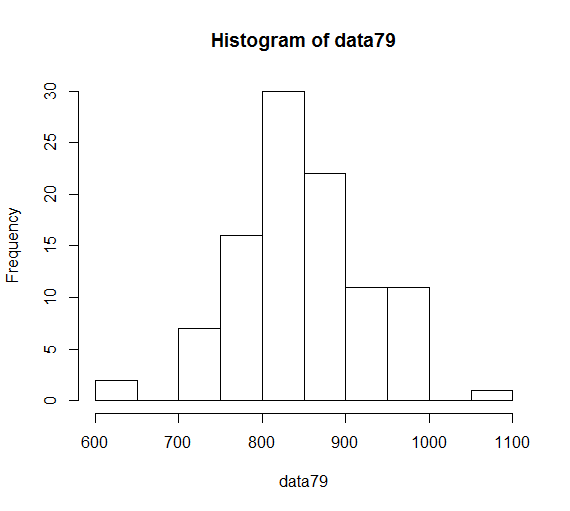
\includegraphics[scale=0.35]{../results/Hist1879.png} }
      \subfigure[1882]
      {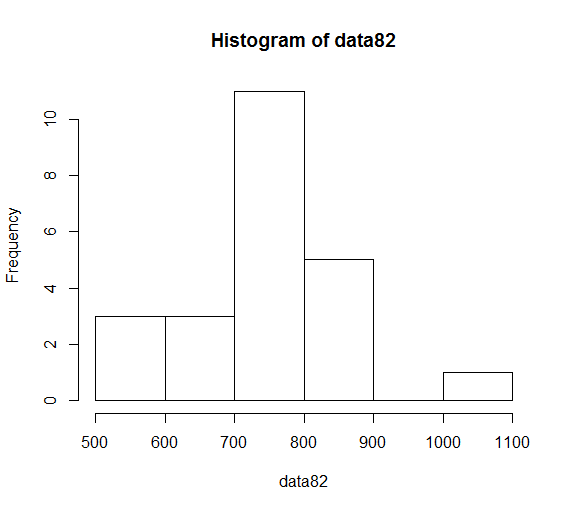
\includegraphics[scale=0.35]{../results/Hist1882.png} }
      \caption{Histograms of the datasets Light1879 and Light1882}
      \label{fig:HistEx2}
    \end{figure}

  \section{Exercise 3}
    In this exercise the klm dataset will be examined.
    This dataset contains data of the duration of deliveries in days.
    In Fig:\ref{fig:GraphKLM} the histogram and boxplot of this dataset are shown.
    Looking at these graphs, it is clear that the dataset is not normally distributed.
    So for hypothesis testing the t-test can't be used, because it assumes the dataset is normally distributed.
    Because of this the sign-test will be used, which can be used for any sort of distribution.
    To test the hypothesis if the meadian duration is smaller than or equal to 35 days,
    the code in Sec:\ref{sec:RE3} is used.
    The results are as follows:\\
    \begin{lstlisting}[language=R]
        One-sample Sign-Test

      data:  klm
      s = 36, p-value = 0.155
      alternative hypothesis: true median is not equal to 35
      95 percent confidence interval:
       32.00000 56.07713
      sample estimates:
      median of x 
               42 

                        Conf.Level L.E.pt  U.E.pt
      Lower Achieved CI     0.9481     32 56.0000
      Interpolated CI       0.9500     32 56.0771
      Upper Achieved CI     0.9727     32 57.0000
    \end{lstlisting}
    This means that H0 is rejected, the median is not equal to 35 but it is 42.\\\\
    To test the hypothesis if at most 10\% of the parts arrives after the maximum delivery period of 70 days,
    the code in Sec:\ref{sec:RE3} is used.
    Now for the test if at most 10\% of the parts arrives after the maximum delivery period of 70 days.
    The self written program can be found in \ref{sec:RE3}.
    The results are as follows:\\
    \begin{lstlisting}[language=R]
        Exact binomial test

      data:  14 and 3464
      number of successes = 14, number of trials = 3464, p-value < 2.2e-16
      alternative hypothesis: true probability of success is not equal to 0.5
      99.5 percent confidence interval:
       0.001661284 0.008114514
      sample estimates:
      probability of success 
                  0.00404157 
    \end{lstlisting}
    This means that H0 is not rejected and that less than 10\% of the parts arrive after 70 days.

    \begin{figure}
      \includegraphics[scale=0.6]{../results/resultKLM.png}
      \caption{Graphs of the dataset klm}
      \label{fig:GraphKLM}
    \end{figure}

  \section{Exercise 4}
    In Fig:\ref{fig:RunBefAf} the data of the before and after the drink running times are visualized.
    Here it is clear that overall the running times where higher after the drink and a bit less normally distributed.
    In Fig:\ref{fig:RunDrink} the before and after times of the two drinks are compared.
    Here you can see that the lemon group had the worst runners in the before the drink and is normally distributed.
    The energy group had a more uniformally distributed before the drink.
    After the drink the lemo drinkers where faster than the energy group, while the name energy drink suggests that you would perform better.

    \begin{figure}
      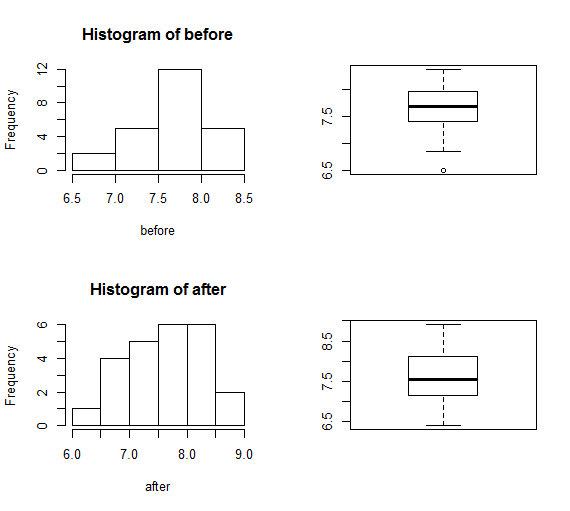
\includegraphics[scale=0.6]{../results/GraphBeforeAfter.png}
      \caption{Histogram and boxplot of the running times before and after the drink}
      \label{fig:RunBefAf}
    \end{figure}
    \begin{figure}
      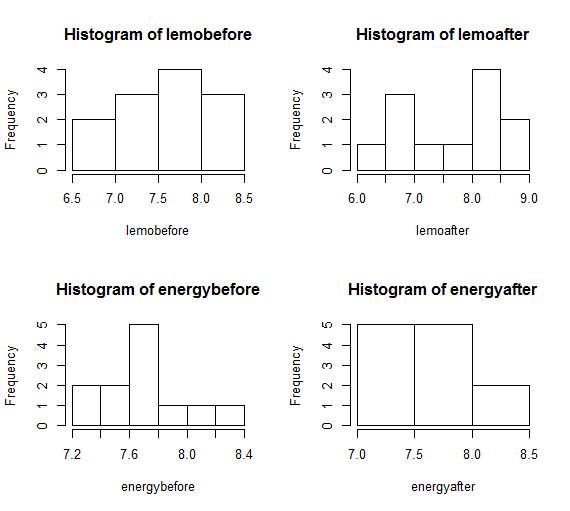
\includegraphics[scale=0.6]{../results/HistLemoEnergy.png}
      \caption{Histograms of the before and after times sorted on the drink}
      \label{fig:RunDrink}
    \end{figure}


  \section{R-Code}
    \subsection{Exercise 1}\label{sec:RE1}
      \begin{lstlisting}[language=R]
      mydata= as.vector(t(dataexp))

	Tstar = numeric(25)
	for(i in 1:25)
	{
	  Xstar = sample(mydata, replace=TRUE)
 	 Tstar[i] = mean(Xstar) - median(Xstar)
	}


	Tstar25 = quantile(Tstar,0.025)
	Tstar975 = quantile(Tstar,0.975)
	T1 = mean(Tstar)
	ans1 = c(2*T1 - Tstar975, 2*T1 - Tstar25)

	test = rexp(25)
	ans2 = mean(test)
	test25 = quantile(test, 0.025)
	test975 = quantile(test, 0.975)
	ans3 = c(2*ans2 - test975, 2*ans2 - test25)
      \end{lstlisting}
    \subsection{Exercise 2}\label{sec:RE2}
      \begin{lstlisting}[language=R]
      data79 = read.table("light1879.txt", header=F)
      data82 = read.table("light1882.txt", header=F)

      #2.1
      data79 = as.matrix(data79)
      hist(data79)
      data82 = as.matrix(data82)
      hist(data82)

      #2.2
      error = qnorm(0.975)*sd(data79)/sqrt(length(data79))
      left = mean(data79)-error
      right = mean(data79)+error
      c(left, right)

      #2.3
      error = qnorm(0.975)*sd(data82)/sqrt(length(data82))
      left = mean(data82)-error
      right = mean(data82)+error
      c(left, right)

      #2.4
      error = qnorm(0.975)*sd(data79)/sqrt(length(data79))
      left = median(data79)-error
      right = median(data79)+error
      c(left, right)

      #2.5
      error = qnorm(0.975)*sd(data82)/sqrt(length(data82))
      left = median(data82)-error
      right = median(data82)+error
      c(left, right)
      \end{lstlisting}
    \subsection{Exercise 3}\label{sec:RE3}
      \begin{lstlisting}[language=R]
      library(BSDA)

      #3.1
      klm = scan(file = "klm.txt")

      par(mfrow=c(1,2))
      hist(klm)
      boxplot(klm)

      SIGN.test(klm, md=35, conf.level = 0.995)

      #3.2
      sum(klm)
      sum(klm > 70)
      binom.test(14,3464,conf.level = 0.995)

      \end{lstlisting}
    \subsection{Exercise 4}\label{sec:RE4}
      \begin{lstlisting}[language=R]
      library(BSDA)

      run = read.table(file = "run.txt")

      #4.1
      before = as.numeric(run[,1])
      after = as.numeric(run[,2])
      par(mfrow=c(2,2))
      hist(before)
      boxplot(before)
      hist(after)
      boxplot(after)

      #4.2
      lemo = run[which(run[,3]=="lemo"), 1:2]
      energy = run[which(run[,3]=="energy"), 1:2]
      lemobefore = as.numeric(lemo[,1])
      energybefore = as.numeric(energy[,1])
      lemoafter = as.numeric(lemo[,2])
      energyafter = as.numeric(energy[,2])
      par(mfrow=c(2,2))
      hist(lemobefore)
      hist(lemoafter)
      hist(energybefore)
      hist(energyafter)
      \end{lstlisting}

\end{document}